\documentclass{report}
\usepackage[utf8]{inputenc}
\usepackage[english]{babel}
\usepackage{apacite}
\usepackage{graphicx}
\usepackage{mathptmx}
\usepackage[font = {small, it}]{caption}
\DeclareCaptionLabelFormat{cont}{#1~#2\alph{ContinuedFloat}}
\captionsetup[ContinuedFloat]{labelformat=cont}
%\usepackage{subcaption}
\usepackage{subfigure}
\usepackage{float}
\usepackage{fancyhdr}

\fancypagestyle{plain}{
\fancyhf{}
\rhead{Mikkel Werling, 201706722}
\lhead{PAPER 2}
\cfoot{\thepage}
}
\pagestyle{plain}

\setlength{\parindent}{2em}
\setlength{\parskip}{1em}
\renewcommand{\baselinestretch}{1.5}


\title{PyCipio: Bayesian Time-series Prediction}
\author{Mikkel Werling\\201706722}
\date{}
\begin{document}%sese
\maketitle
\section{Introduction}

\begin{figure}[ht]
    \centering
    \subfigure[First plot]{%
        \label{fig:supfigure1}
        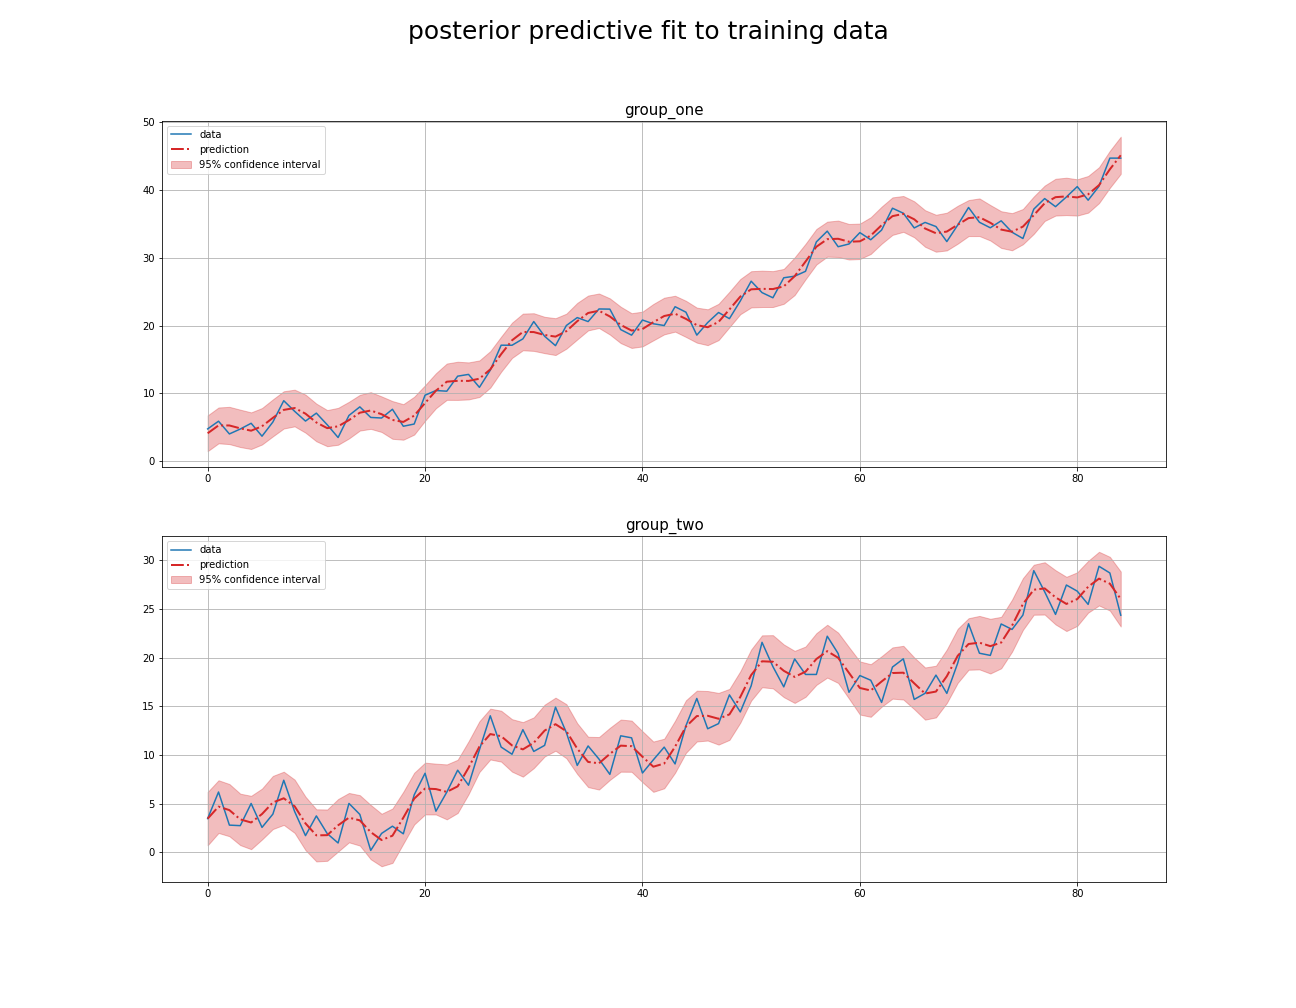
\includegraphics[width = 0.45 \textwidth]{../plots/ex1_plot_fit_idx_all}}
    \quad
    \subfigure[Second plot]{%
        \label{fig:supfigure2}
        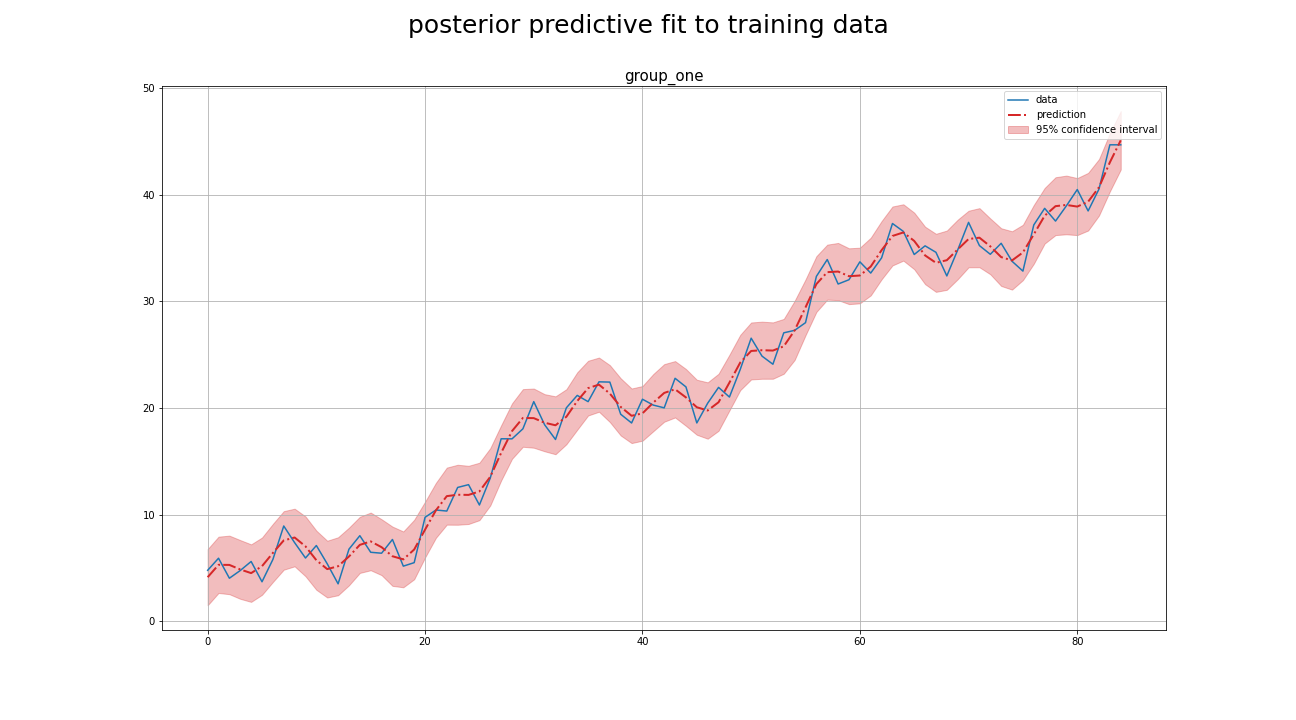
\includegraphics[width = 0.45 \textwidth]{../plots/ex1_plot_fit_idx_single}}
    \subfigure[Third Plot]{%
        \label{fig:supfigure3}
        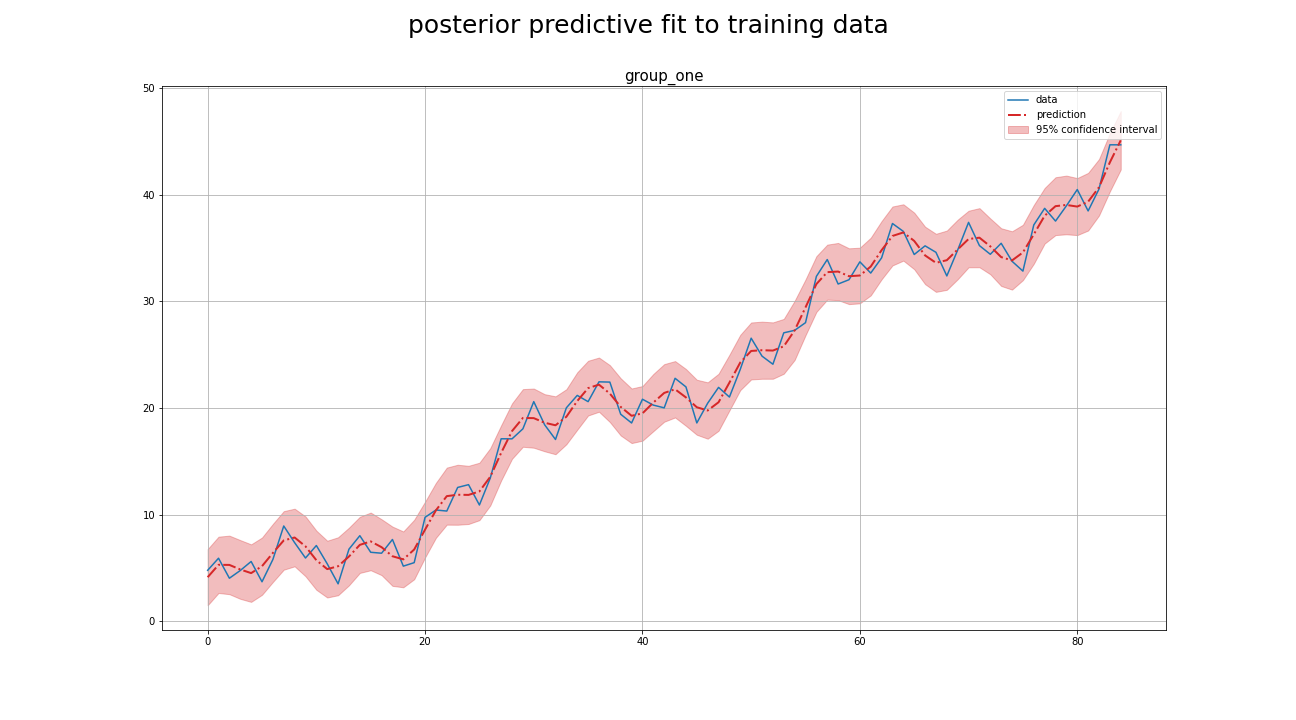
\includegraphics[width = 0.45 \textwidth]{../plots/ex1_plot_fit_idx_single}}
    \quad
    \subfigure[Fourth plot]{%
        \label{fig:supfigure4}
        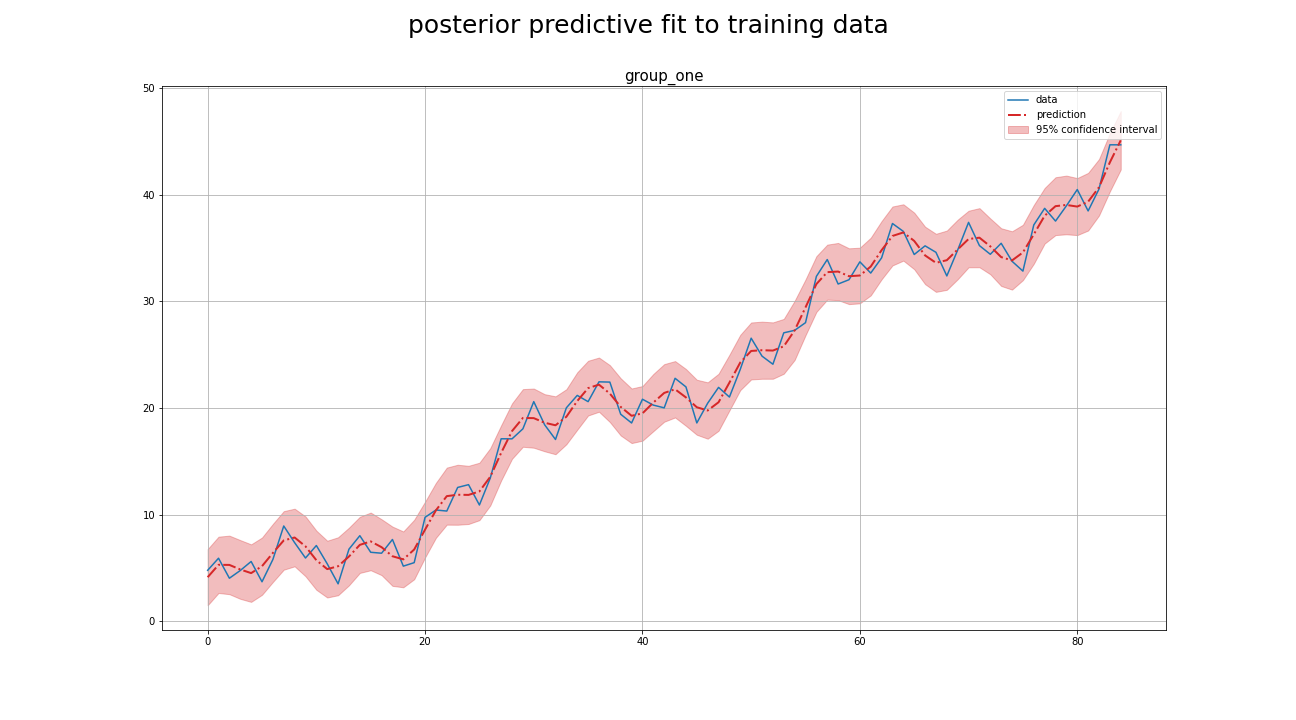
\includegraphics[width = 0.45 \textwidth]{../plots/ex1_plot_fit_idx_single}}
    
    \caption{Predictions in one and 2 groups}
\end{figure}


%\bibliographystyle{apacite}

%\bibliography{cite2}

\end{document}